\documentclass[xcolor={dvipsnames}]{beamer}
%  \usetheme{JuanLesPins}
   \usetheme{Boadilla}
%   \setbeamertemplate{frametitle continuation}[from second]
%   \setbeamertemplate{bibliography entry title}{}
%   \setbeamertemplate{bibliography entry location}{}
%   \setbeamertemplate{bibliography entry note}{}
\usepackage[utf8]{inputenc}
\usepackage[english]{babel}
\usepackage{alltt}
\usepackage{graphicx}

%\usepackage{etex}
%\usepackage{ulem}
%\usepackage[all]{xy}
%\usepackage{tikz}
%\normalem
%\usepackage{alltt}
%\usepackage{fancyvrb}
%\usepackage{hyperref}
%\usepackage{pdfpages}
%\usepackage{comment}
\usepackage{booktabs}
%
%\usepackage{listings}
%\usepackage{algorithmic}
%\usepackage{datatool}
%
%
%%\usepackage{mathpartir}
%\usepackage{algorithmic}
%\usepackage{wasysym}

%\input{macros}

%\graphicspath{{pics/}{pics/logos/}} % Root directory of the pictures

%\input{macros}

\newcommand{\ZZZ}[1]{\textcolor{red}{#1}}
\newcommand{\EEE}[1]{\textcolor{BlueViolet}{#1}}

\title[Comigrate]%
{Comigrate: \\ improving package migration \\
 from \texttt{unstable} to \texttt{testing}}

\author[Di Cosmo/Dogguy/Vouillon]{Mehdi Dogguy, J\'er\^ome Vouillon and Roberto Di Cosmo}

\date[2014-01-18]{January 18, 2014}

\begin{document}

\begin{frame}[label=title]{}
 \titlepage
 \vspace{-1.5cm}
 \begin{center}
%  
\includegraphics[width=1cm]{p7} \hfill
%  
\includegraphics[width=2.5cm]{inria-logo-new} \hfill
%  
\includegraphics[width=2.5cm]{Logotype-IRILL} \hfill
%  
\includegraphics[width=1.5cm]{cnrsfilaire_quadri} \hfill
 \end{center}
\end{frame}

\begin{frame}{Introduction}

\EEE{Comigrate}

Tool designed to help package integration in Debian \textit{testing}.

\vspace{3em}

\EEE{Talk outline}
\begin{itemize}
\item Package integration process
\item History of \texttt{comigrate}
\item Presentation of \texttt{comigrate}
\end{itemize}
\end{frame}

\part{Package migration}
\frame{\partpage}

\begin{frame}{Package Migration}

\begin{center}
\includegraphics[width=0.7\linewidth]{figures/migration}
\end{center}

\vspace{-1em}
\EEE{Conflicting goals}
\begin{itemize}
\item package should reach \textit{testing} rapidly
\item keep \textit{testing} as stable as possible
\end{itemize}

\end{frame}

\begin{frame}{Conditions for migration}
\EEE{Simple constraints} % (Boolean constraints):
\begin{itemize}
\item old enough
\item no new critical bug
\item simultaneous migration of source and binary packages
\item ...
\end{itemize}

\vspace{1em}

\EEE{Complex constraints}
\begin{itemize}
\item packages in \textit{testing} should remain installable
%\item (packages should remain co-installable)
\end{itemize}
\end{frame}

\begin{frame}{Britney}

\EEE{Compute which packages can migrate}
\begin{enumerate}
\item find a list of migration candidates (simple constraints)
\item check whether migrating these candidates preserve installability
\begin{itemize}
\item first, check each candidate in isolation
\item then, try cluster of candidates (heuristics)
\end{itemize}
\item output the migration outcome
\end{enumerate}

\vspace{1cm}

\EEE{Hint mechanism}
\begin{itemize}
\item override default behavior (block packages / force migration)
\item indicate cluster of packages that can migrate together
\end{itemize}
\end{frame}

\begin{frame}[fragile]{Shortcomings of Britney}

\EEE{Can fail to migrate automatically some packages}

Heuristic-based

\vspace{1.5em}

\EEE{Complex migrations are hard to debug}

\begin{itemize}
\item OCaml transition:
200 source packages involved (hint with about 1300 elements)
\item KDE transition: 150 source packages
\end{itemize}
%An issue in any of these packages will prevent the migration of all of them!
Limited help provided by Britney to find issues.
\begin{itemize}
\item what packages are involved?
\item which of them have issues?
\end{itemize}

\vspace{1.5em}

\EEE{Preserving installability might not be enough...}

Trade-off: more work for the release team / better quality

\iffalse
\begin{quote}
\begin{verbatim}
trying: apr-util
skipped: apr-util (801 <- 513)
    got: 3+0: i-3
    * i386: libaprutil1-dbd-freetds
\end{verbatim}
\end{quote}
\fi

\end{frame}

\begin{frame}[fragile]{Transient incompatibilities}

\begin{alltt}
[2013-10-16] icedove 17.0.9-2 MIGRATED to testing
[2013-11-25] enigmail 2:1.6-4 MIGRATED to testing
\end{alltt}

Bug \#726517 ---  enigmail: uninstallable in jessie due to FTBFS
\begin{quote}
the current version of enigmail in sid won’t migrate to jessie
because of an FTBFS (on kfreebsd). \EEE{A version of icedove which
is incompatible with the old version of enigmail migrated to
jessie today.}
\end{quote}

\vspace{0.5em}

\begin{alltt}
[2013-08-01] kfreebsd-9 9.1-4 MIGRATED to testing
[2013-10-11] grub2 1.99-27+deb7u2 MIGRATED to testing
\end{alltt}

\begin{alltt}
Package: kfreebsd-image-9.2-1-amd64
Breaks: grub-common (<< 1.99-27+deb7u2)
\end{alltt}

\end{frame}

\begin{frame}{Debian testing: conflict \texttt{libhfd5} -- \texttt{libhdf5-openmpi-7}}

\EEE{Depend on libhdf5-openmpi-7:} libmed1, libpetsc3.2, code-saturne
libsiloh5-0, libslepc3.2, libxdmf2, syrthes, fenics, cdo[non i386]

\vspace{0.5em}

\EEE{Depend on libhdf5-7:} libmapnik-dev, libhe5-hdfeos-dev
grass-dev, liblas-dev, libgdal-dev, libqgis-dev

\vspace{2em}

Bug \#689426 --- libgdal-dev: depend on other libhdf flavors?
\begin{quote}
Dear Maintainer, 
installing libgdal-dev on my system would remove a lot of packages: [...]
\end{quote}
Bug \#712829 --- cdo depends on libhdf5-openmpi-dev; should depend on libhdf5-dev
\begin{quote}
Dear Maintainer,
cdo and libgdal1-dev cannot be installed together [...].
This is obviously a fairly serious
problem.
\end{quote}

\end{frame}

\begin{frame}
\texttt{tesseract-ocr} incompatible with \texttt{tesseract-ocr-en}
\begin{center}
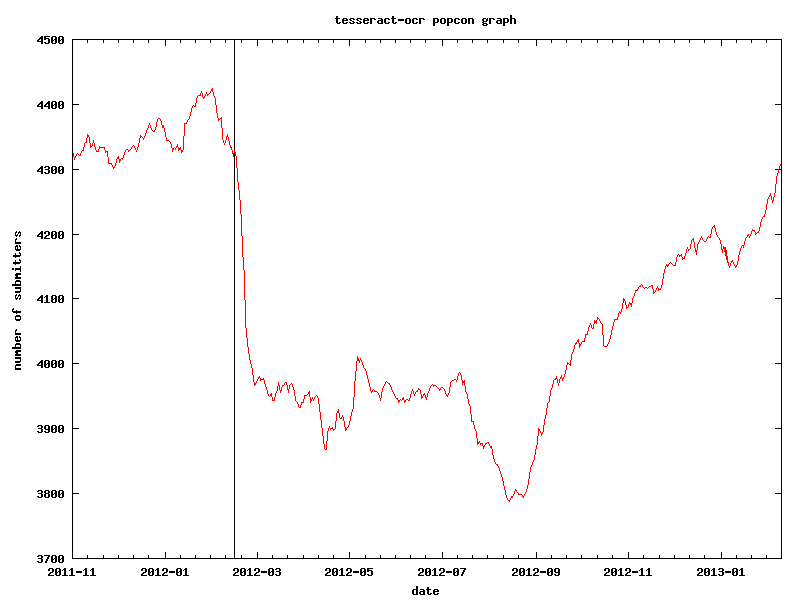
\includegraphics[width=0.8\linewidth]{figures/tesseract-ocr}
\end{center}
\end{frame}

\begin{frame}
\texttt{openclipart-libreoffice} incompatible with \texttt{libreoffice}
\begin{center}
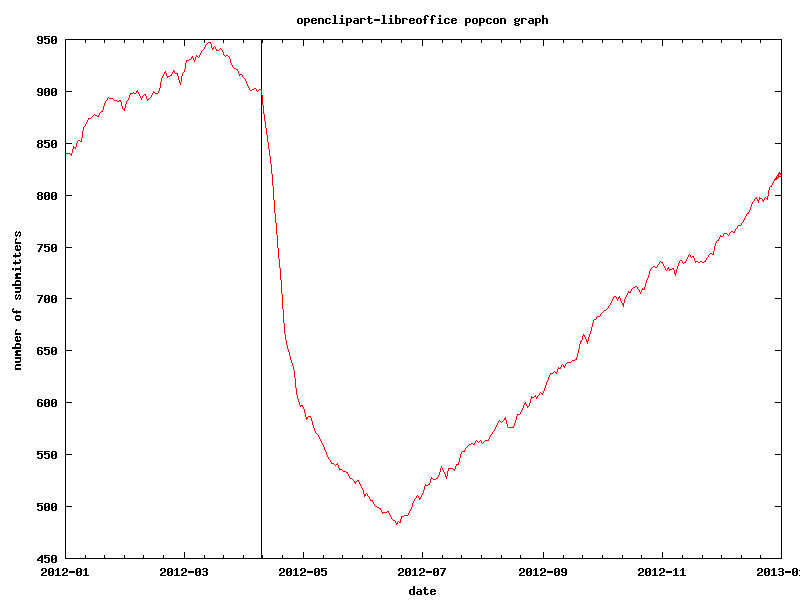
\includegraphics[width=0.8\linewidth]{figures/openclipart-libreoffice}
\end{center}
\end{frame}

\part{History of comigrate}
\frame{\partpage}

\begin{frame}{Global goal}

\EEE{Analyze conflicts between packages}
\begin{itemize}
\item what packages cannot be installed at all
\item what are the incompatibilities between packages
\item how these incompatibilities evolves
\item ... and finally, package migration
\end{itemize}

\end{frame}

\begin{frame}{Package installability}

List all packages which cannot be installed at all in a repository.
\texttt{debcheck}

Now, package \texttt{dose-distcheck}

Debian Weather (down?)
\url{http://edos.debian.net/weather/}

\url{http://qa.debian.org/debcheck.php}

Clear expectation: all packages should be installable

\end{frame}

\begin{frame}[fragile]{Co-installability}
\EEE{Definition:} a set of packages are co-installable if they can be install
together.

\vspace{1.5em}
Package incompatibilities are to be expected.
%
How do we visualize them?

See \url{http://coinst.irill.org/}
\end{frame}

\begin{frame}[fragile]{Co-installability graphs}
\begin{alltt}
coinst -root \EEE{iceweasel} -o graph.dot Packages_i386
\end{alltt}
\vspace{-2.5em}
\begin{center}
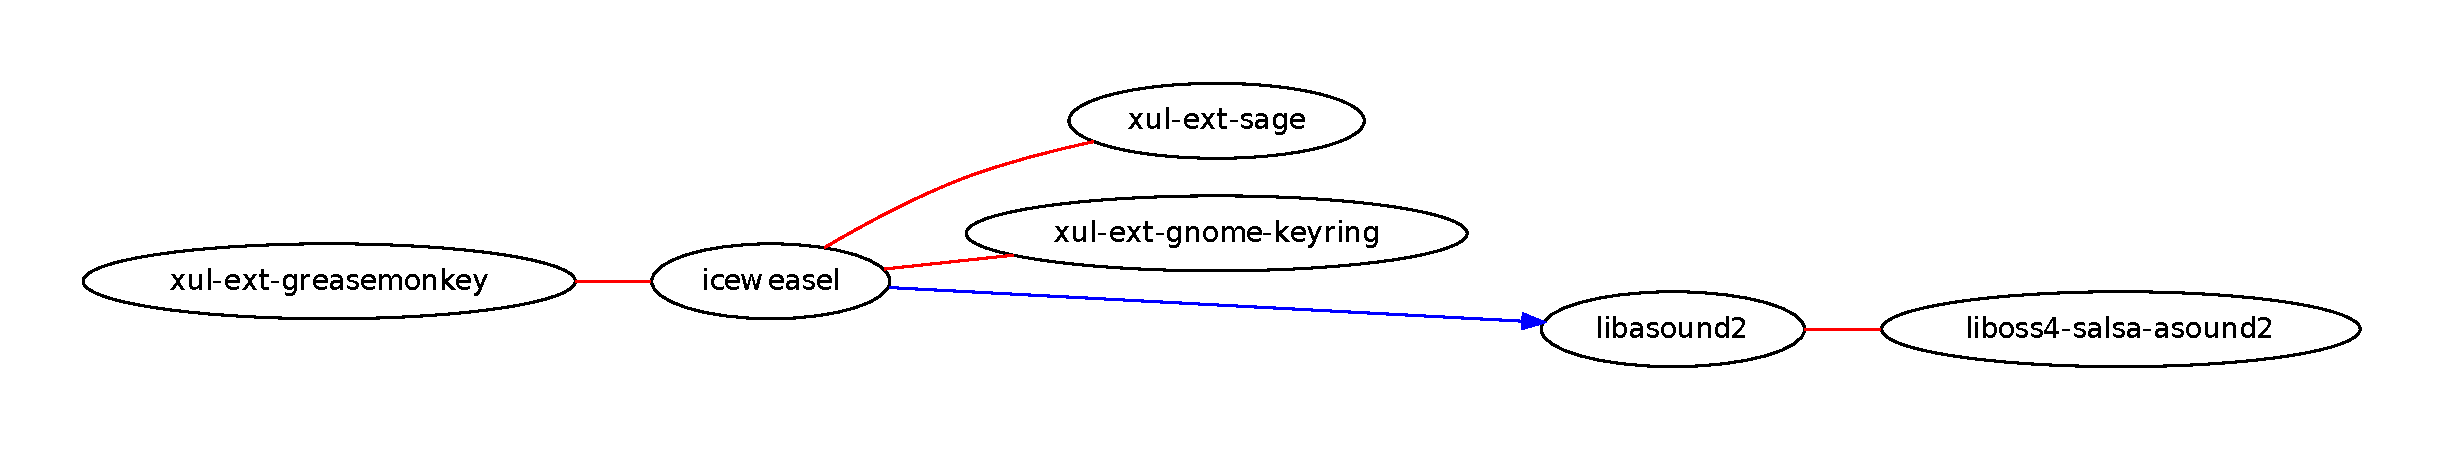
\includegraphics[width=\linewidth]{figures/iceweasel.pdf}
\end{center}
\vspace{-2em}
\begin{alltt}
coinst -root \EEE{kde-full} -o graph.dot Packages_i386
\end{alltt}
\vspace{-2.5em}
\begin{center}
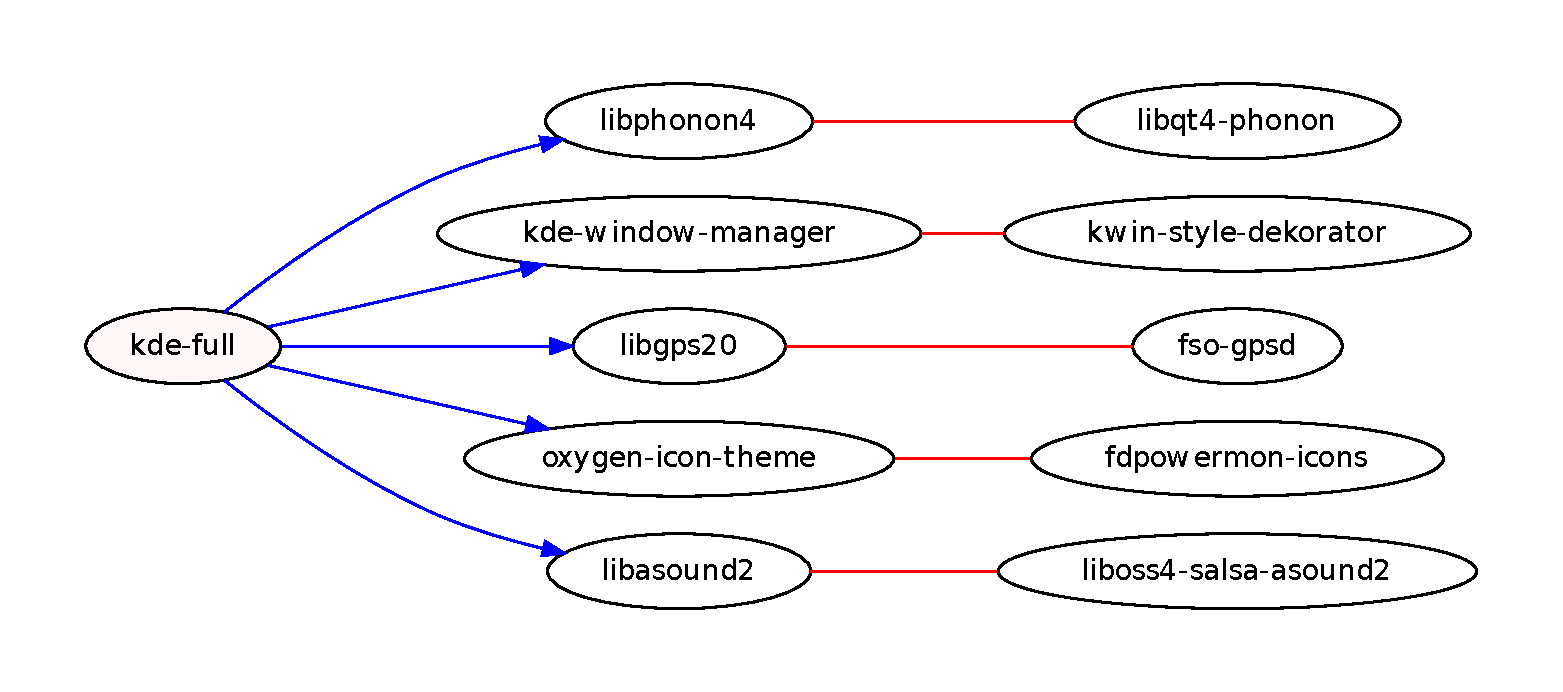
\includegraphics[width=0.65\linewidth]{figures/kde-full.pdf}
\end{center}
\end{frame}

\begin{frame}
\begin{center}
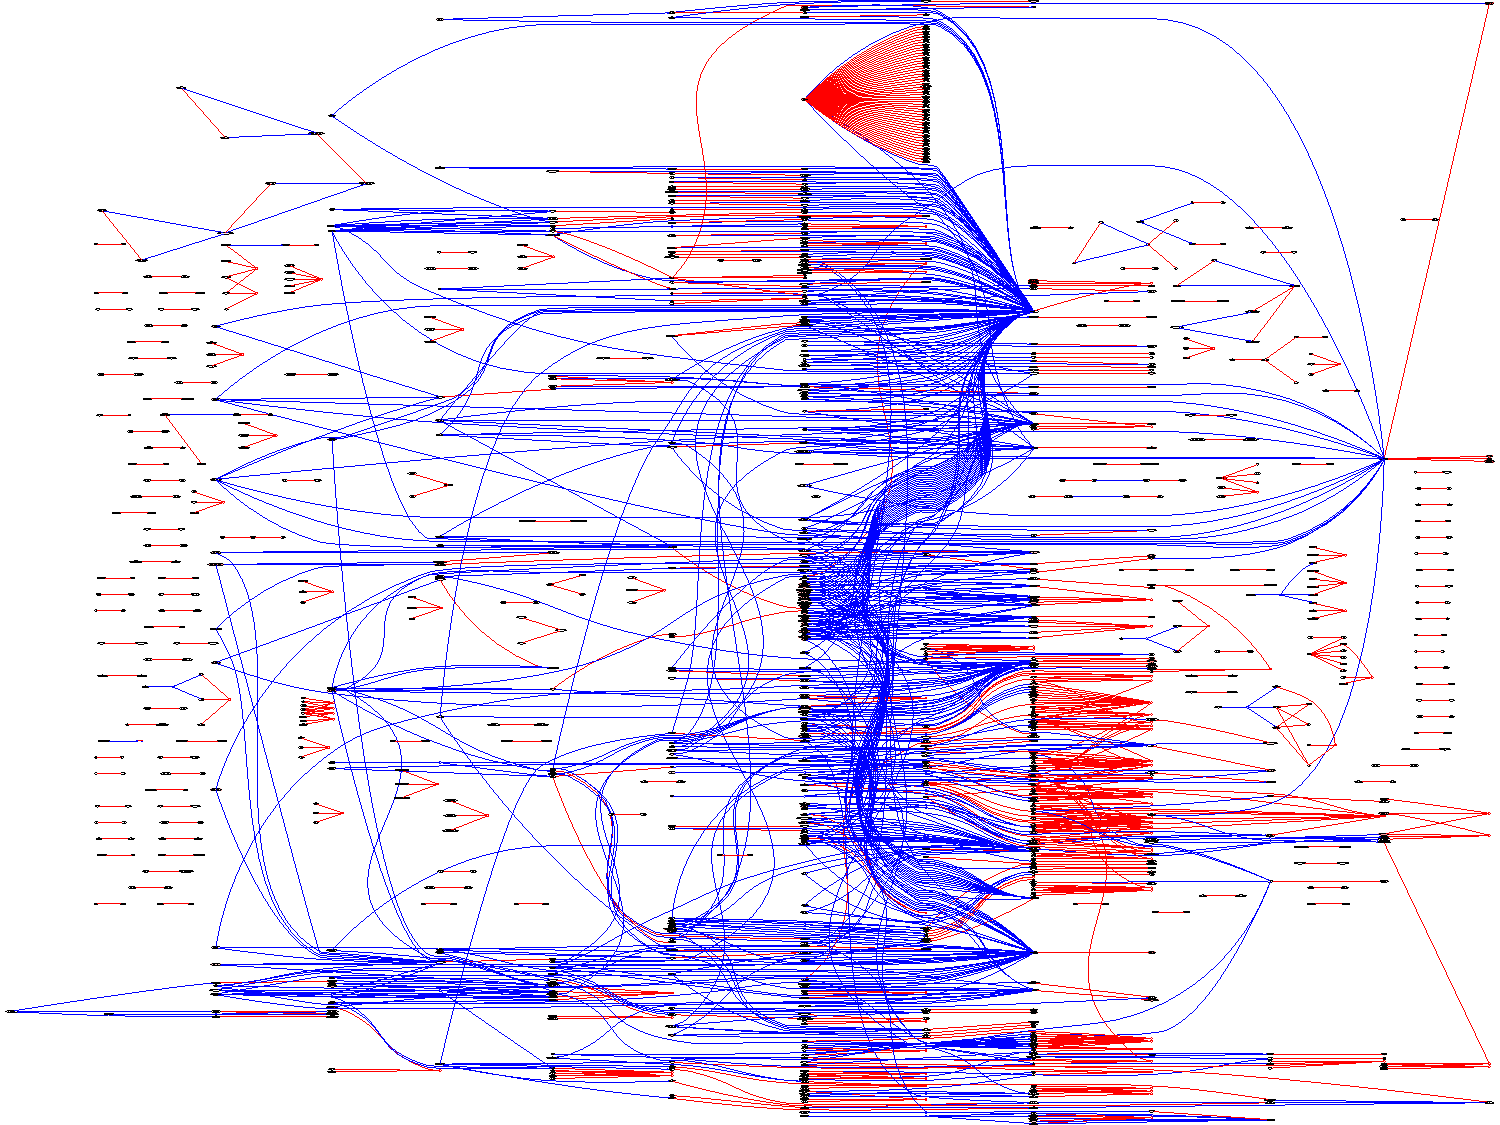
\includegraphics[width=\linewidth]{figures/flattened}
\end{center}
\end{frame}

\begin{frame}{Co-installability: algorithm}
\EEE{Key ideas}
\begin{itemize}
\item Transitive closures of package dependencies
\item Remove dependencies that can always be satisfied
\end{itemize}

\begin{center}
\begin{tabular}{@{}lrrrrrr@{}}
\toprule
& Before & After \\
\midrule
Packages & 28919 & 1038 \\
Dependencies & 124246 & 619 \\
Conflicts & 1146 & 985 \\
Median cone size & 38 & 1 \\
Avg. cone size & 66 & 1.7 \\
Max. cone size & 1134 & 15 \\
\midrule
Running time
& & 10.6 seconds
\\
\bottomrule
\end{tabular}
\end{center}

\end{frame}

\begin{frame}{Finding new co-installability issues}
\url{http://coinst.irill.org/upgrades}

find new issues

\begin{description}
\item[For the Debian maintainers:]
are there any dependency-related bugs introduced recently? since the
last stable release?
\item[For the end-user:] will I have any issue upgrading my system?
\end{description}

XXX Need to give an intuition of what we compute
(graph with quadratic number of conflicts?)

Important present properly these issues (KDE example)

\begin{center}

\includegraphics{figures/libiodbc2}
\end{center}

\texttt{libiodbc2} is obsoletes

\end{frame}

\begin{frame}{Context}
\begin{center}

\includegraphics{figures/libiodbc2}
\end{center}
Depend on \texttt{libiodbc2} (about 380 package):
kcolorchooser kdesdk-misc kdevelop-php-docs blinken kdevelop
kmousetool ktorrent kalgebra konqueror klipper kchmviewer
mplayerthumbs libsmokekutils3 kjots ksshaskpass cantor
network-manager-kde kbattleship choqok kdesdk-dbg krusader-dbg
libkdegames-dev kmidimon klettres quassel-kde4 libakonadi-ruby
konq-plugins ktorrent-dbg kiriki plasma-widgets-workspace kvirc-dbg
konversation-dbg libkiten-dev kdm-gdmcompat plasma-netbook
libokular-ruby1.8 eqonomize kdenetwork-dbg libsmokeplasma3 kspread
lokalize korganizer parley kfourinline libsmokekde-dev kfind
kdepim-groupware ksnapshot libiodbc2-dev plasma-runners-addons
libsmokekdeui4-3 printer-applet ark kdeutils kover rocs kdesvn-dbg
kdevplatform-dev libkdepim4 ktron cantor-backend-sage kinfocenter
kjumpingcube kaddressbook kmymoney akonadiconsole cantor-backend-r
kmines kgoldrunner partitionmanager libsublime-dev korundum4
kphotoalbum kplayer
\ldots

\end{frame}

\part{Comigrate}
\frame{\partpage}

\begin{frame}{Applications}

\begin{itemize}
\item \EEE{Interactively investigate migration issues}

Run it repeatedly, studying different scenarios

\vspace{0.5em}

\item \EEE{Supplement Britney}

Generate hints that can be feed to Britney

\vspace{0.5em}

\item \EEE{Report of issues preventing package migration}

\url{http://coinst.irill.org/report/}

\end{itemize}
\end{frame}

\begin{frame}{Tool architecture}

\vspace{-1em}
\begin{center}
\includegraphics[width=0.5\linewidth]{figures/architecture}
\end{center}

\vspace{-1em}

\begin{itemize}
\item Start with simple constraints
\item The Boolean solver generates a tentative migration
\item 
 Check for (co-)installability issues;
  analyse these issues to generate new constraints
  (``package \texttt{A} cannot migrate'',
  or ``package \texttt{A} cannot migrate without package \texttt{B}'')
\item Repeat until no more issue is found
\end{itemize}
\end{frame}

\begin{frame}{Performance}

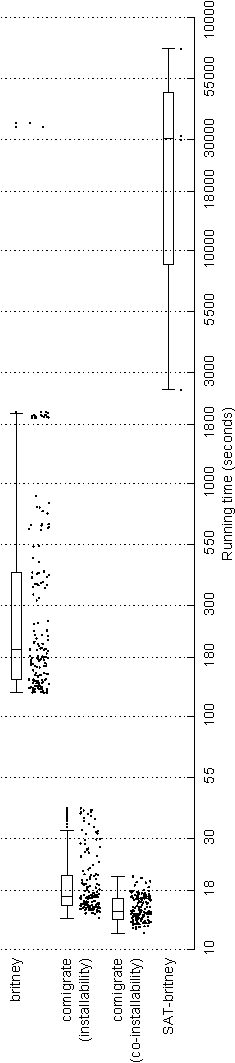
\includegraphics[height=\linewidth,angle=-90]{figures/performance.pdf}

\vspace{2em}

\scriptsize
Data collected twice a day from 2013-06-24 to 2013-09-09
\end{frame}


\begin{frame}{Ressources}

\EEE{Tool information:} \url{http://coinst.irill.org/comigrate}

\vspace{1em}

\EEE{Source code:} \url{https://github.com/vouillon/coinst}

\vspace{1em}

\EEE{Packages:} \texttt{dose-distcheck}, \texttt{coinst}, and
\texttt{coinst-viewer} in Debian. Other tools forthcoming.

\vspace{1em}

\EEE{Daily report:}
\url{http://coinst.irill.org/report}
\end{frame}

\end{document}
